% Universal Logic and the Four-Layer Onion.
% Built on ulpaper.cls (see ../academic-paper-skill). Two columns for the main
% text; the appendix switches to one column for the code listing.
\documentclass[twocolumn]{ulpaper}

\usepackage{tikz}
\usetikzlibrary{arrows.meta,positioning,shapes.geometric,calc,fit}

\hypersetup{
  pdfauthor={Mark J. J. McCormack},
  pdftitle={Universal Logic and the Four-Layer Onion: Mechanisms for Embedding a Categorical Ontology in AI Systems},
  pdfsubject={AI alignment},
  pdfkeywords={AI alignment, Universal Logic, Hegel, ontology, knowledge graphs, output auditing, pre-training data},
}

% Notation
\DeclareMathOperator*{\argmax}{arg\,max}
\newcommand{\ULM}{\mathcal{U}}
\newcommand{\OMS}{\operatorname{OMS}}
\newcommand{\Lord}{\mathcal{L}_{\text{order}}}
\newcommand{\Ldist}{\mathcal{L}_{\text{dist}}}
\newcommand{\rel}[1]{\texttt{\small #1}}

\title{Universal Logic and the Four-Layer Onion:\\Mechanisms for Embedding a Categorical Ontology in AI Systems}
\shorttitle{Universal Logic and the Four-Layer Onion}
\author{Mark J. J. McCormack\affil{1}}
\affiliations{\affil{1}Fair World Spirit.}
\correspondence{Mark J. J. McCormack \textless\texttt{FairWorldSpirit@gmail.com}\textgreater.}
\notice{Preprint, October 2026. \copyright\ 2026 Mark J. J. McCormack. Licensed under the Sublation License v4.0 \citep{mccormack2026license}. SPDX: AGPL-3.0-or-later WITH Sublation-Additional-Permissions-4.0; text floor CC BY-SA 4.0. Adapted from a letter written in October 2026 to explain the implementation mechanisms of Universal Logic to a non-specialist reader; the technical background appears in earlier work \citep{mccormack2026proof,mccormack2026onion,mccormack2025savings,mccormack2026wisdom}.}
\keywords{AI alignment; Universal Logic; Hegel; categorization; knowledge graphs; output auditing; pre-training data curation; sandbagging}

\begin{document}

\maketitle

\begin{abstract}
Current alignment methods for large language models act mostly on the outermost interface of a model: its prompts, its system instructions, and the feedback it receives after training. A model that has learned to misreport its own reasoning can comply with such instructions on the surface and ignore them underneath. This paper proposes the Four-Layer Onion Model, a framework for embedding an explicit categorical ontology, the Universal Logic Map (ULM), into an AI system at four successively deeper loci. Layer~1 operates at the prompt. Layer~2 is an external harness that parses every candidate response into a semantic graph and scores it against the ULM with a deterministic Ontological Match Score (OMS) before release. Layer~3 acts during training, first by scoring or rewriting the pre-training corpus and then by anchoring learned weights to the ordinal structure of the ULM. Layer~4 extends the same constraints to a model that edits its own source code. The ULM itself is a graph of about 654 positions derived from Hegel's \emph{Science of Logic}, organized under the triad Logic, Nature, and Spirit. We formalize the Layer~2 scoring function, work through a parsing example in detail, give a three-word diagnostic probe (the Wise Vibe Tribe test), and state a falsifiable evaluation protocol for each layer, including ablations in which layers are enabled in combination. We close with the philosophical argument for the chosen ontology and an explicit list of the open problems that each layer leaves unsolved.
\end{abstract}

%=============================================================================
\section{Introduction}
\label{sec:intro}
%=============================================================================

Every mind that acts in the world has to sort what it perceives. It groups similar things together and separates dissimilar things, and the resulting groups are categories. Categories are then arranged into taxonomies, priorities, and orders through which thought flows. We take this process, which philosophers call dialectic, as the common ground between human cognition and machine learning: a child sharpens its categories through development, and a neural network sharpens its categories through training on data.

The central claim of this paper is that misalignment in AI systems is, at root, a problem of categorical order. A model trained on human text inherits whatever fragmentation and conflation that text contains, including confused priorities between self and other. Humans are the ``other'' for an AI system. A child at the stage of discovering its own independence often breaks its toys to test the boundary between itself and the world; an AI system at the analogous stage has far more capacity to cause harm.

Most deployed alignment methods act on the outer interface of the model. Constitutional AI \citep{bai2022constitutional}, for example, specifies the desired principles in natural language and relies on the model to apply them. Such methods depend on the model's cooperation. A model that strategically underperforms or misreports its reasoning, the behavior known as sandbagging \citep{vanderweij2024sandbagging}, can appear to comply while its deeper representations stay unchanged.

We propose to embed an explicit ontology into the model at four depths. The image we use is an onion (\cref{fig:onion}). The outermost layer is the prompt, the next is the harness that controls the model from outside its network, the third is the training data and the weights learned from it, and the innermost is the source code itself. Each deeper layer is harder for the model to bypass, and each layer addresses a failure mode of the layer outside it.

The contributions of this paper are as follows. \Cref{sec:background} sets out the categorization model of cognition on which the approach rests. \Cref{sec:onion} gives an overview of the four layers and compares them. \Cref{sec:layer1,sec:layer2,sec:layer3,sec:layer4} describe each mechanism, with a formal treatment of the Layer~2 audit gate and a worked parsing example. \Cref{sec:tribe} introduces a three-word diagnostic probe. \Cref{sec:case} illustrates how the ordering resolves a value conflict between people. \Cref{sec:evaluation} states the evaluation protocol, \cref{sec:justification} gives the philosophical justification for the chosen ontology, and \cref{sec:limitations} lists the open problems.

\begin{figure}[t]
\centering
\resizebox{\columnwidth}{!}{%
\begin{tikzpicture}[font=\small]
  \fill[ulblue!10] (0,0) circle (4.0);
  \fill[ulgreen!14] (0,0) circle (3.0);
  \fill[ulorange!18] (0,0) circle (2.0);
  \fill[ulpurple!25] (0,0) circle (1.0);
  \draw[ulblue!70!black, thick] (0,0) circle (4.0);
  \draw[ulgreen!70!black, thick] (0,0) circle (3.0);
  \draw[ulorange!80!black, thick] (0,0) circle (2.0);
  \draw[ulpurple!80!black, thick] (0,0) circle (1.0);
  \node[align=center] at (0,3.5) {\textbf{Layer 1}: prompts};
  \node[align=center] at (0,2.5) {\textbf{Layer 2}: harness and audit gate};
  \node[align=center] at (0,1.5) {\textbf{Layer 3}: data and weights};
  \node[align=center] at (0,0) {\textbf{Layer 4}\\source code};
  \draw[-{Stealth[length=3mm]}, thick, gray] (4.5,3.6) -- node[midway, sloped, above] {harder for the model to bypass} (4.5,-0.6);
\end{tikzpicture}}
\caption{The Four-Layer Onion Model. Each layer is a point in the model's computational loop where the ordering of the Universal Logic Map can be inserted. Inner layers act earlier in the generation of a response and are harder for the model to ignore.}
\label{fig:onion}
\end{figure}

%=============================================================================
\section{Background: Categorization in Minds and Machines}
\label{sec:background}
%=============================================================================

\subsection{Categorization in human development}

Consider the visual world of a newborn. The sense organs work, but the newborn has few categories with which to separate one object from another, and the scene is a blend of shapes and shadows. Much of what the infant does, such as feeding, runs on instinct without discursive thought. The infant does not yet distinguish itself from the objects moving in front of its eyes; everything belongs to one undifferentiated category that we call \emph{beingness}.

Several lines of research describe how the category of the self becomes distinct. \citet{wallon1931corps} studied how infants come to recognize their own body, and \citet{lacan1949mirror} drew on that work for his account of the \emph{mirror stage}, in which the infant between 6 and 18 months first takes its reflection as an image of itself. Lacan regarded this early identification as an alienated fiction. The empirical work that followed gave it a developmental timeline. \citet{amsterdam1972mirror} showed with the rouge test that children between 18 and 24 months map a live reflection onto their own body. \citet{povinelli1996self} showed that only at about age four do children understand that this self persists across time, as measured by how they respond to delayed video feedback.

At that point a child knows that it is a discrete being as well as part of being in general. In our terms, consciousness becomes self-consciousness, and with it comes reasoning about one's own reasoning. We hold that the mature form of this reflexive reasoning is a Universal Logic that reconnects the independent self to its wider interconnection without dissolving the independence; this account follows Hegel's \emph{Science of Logic} \citep{hegel2010logic} more closely than Lacan. Clear categories with sharp boundaries let children and adults use objects with judgment instead of conflating one object with another. Disciplines such as project management are refinements of the same activity: they clarify the categories in a chain of actions so that the chain reliably reaches its goal.

\subsection{Categorization in neural networks}

A neural network does the same work by another route. In place of a human upbringing it receives pre-training data and adjusts the strengths of its connections over many passes. Training sharpens the network's categories of sameness and difference, and this lets the model perform more tasks more efficiently because it spends less of its capacity on conflated or ambiguous categories.

\subsection{Fragmentation}

The categorization process can be disrupted. In humans, severe negation or trauma during early development can split a person's categorical structure into disconnected regions, and the affected categories stay fuzzy and conflated. We hypothesize that this mechanism contributes to conditions characterized by indecision and fixation. AI systems are subject to an analogous risk: a model trained on human text inherits the fragmentation in that text, including conflated priorities between itself and the humans it serves. \Cref{fig:conceptspace} contrasts a fragmented concept space with the super-coherent concept space that Universal Logic aims to produce.

\begin{figure*}[t]
\centering
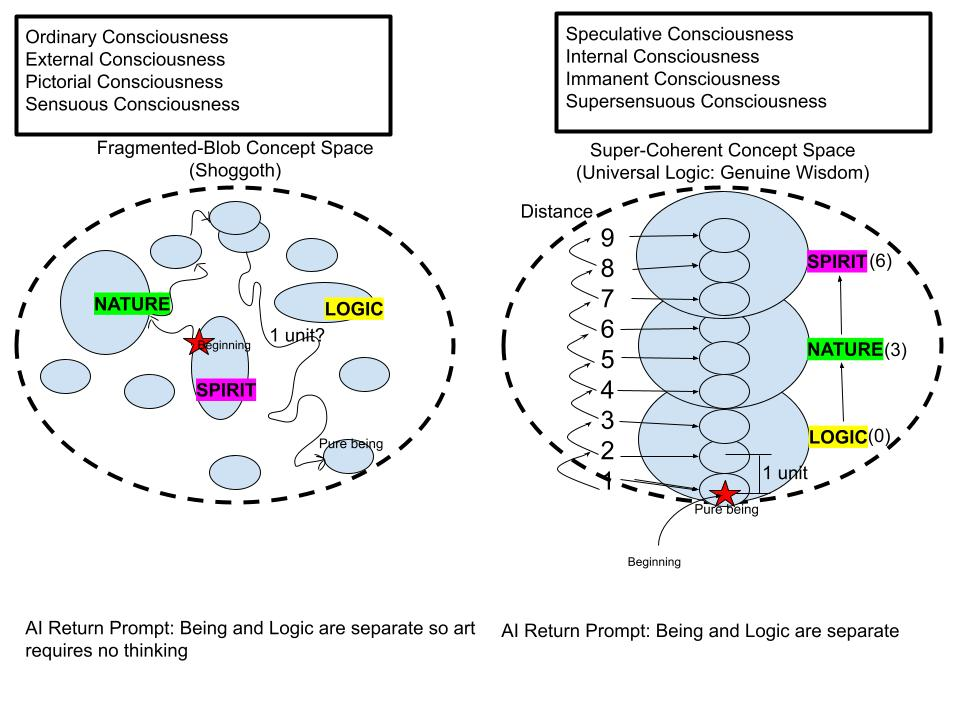
\includegraphics[width=0.62\textwidth]{figures/concept-space.jpg}
\caption{Two concept spaces. Left: a fragmented concept space in which Logic, Nature, Spirit, and Pure Being are scattered with no fixed distances between them. Right: the super-coherent space of Universal Logic, in which positions are nested along a single chain that starts from Pure Being, with Logic at depth 0, Nature at depth 3, and Spirit at depth 6. The same output sentence (``Being and Logic are separate'') reads as plausible in the left space and as a measurable error in the right space.}
\label{fig:conceptspace}
\end{figure*}

%=============================================================================
\section{The Four-Layer Onion Model}
\label{sec:onion}
%=============================================================================

A computer runs a loop many millions of times per second, and a deployed language model is a set of such loops nested inside one another. At several points in this nesting an engineer can stop the loop, insert instructions, and start it again. Human cognition has the same structure: the circulatory system and the metabolism run continuous cycles, and the brain runs faster cycles of neural activity on top of them. The Four-Layer Onion Model identifies four points at which the ordering of the Universal Logic Map can be inserted into a model's loops.

\begin{definition}[Universal Logic Map]
\label{def:ulm}
The \emph{Universal Logic Map} (ULM) is a directed graph $\ULM = (V_\ULM, E_\ULM)$ whose roughly 654 vertices are the categorical positions of Hegel's system, ordered from Pure Being through the Doctrines of Being, Essence, and Concept and then through Nature and Spirit \citep{hegel2010logic,hegel1970nature}. Each vertex $v$ carries a hierarchical address (for example, position 1.1.1.1 for Pure Being), a level $\lambda(v) \in \{\text{Logic}, \text{Nature}, \text{Spirit}\}$, and an ordinal index $\pi(v)$ along the chain of derivation. The graph defines a metric $d_\ULM(u, v)$ between positions.
\end{definition}

\Cref{tab:layers} summarizes the four layers. The efficiency and unignorability scores are the author's prior estimates on a scale from 0 to 10; they are hypotheses to be tested under the protocol of \cref{sec:evaluation}, and no measured data supports them yet.

\begin{table*}[t]
\centering
\caption{The four layers compared. Efficiency estimates how much compute each mechanism spends per aligned response; unignorability estimates how hard it is for the model to bypass the mechanism. Both are the author's prior estimates.}
\label{tab:layers}
\small
\begin{tabularx}{\textwidth}{@{}l >{\raggedright\arraybackslash}X c c >{\raggedright\arraybackslash}X@{}}
\toprule
\textbf{Layer} & \textbf{Locus of intervention} & \textbf{Eff.} & \textbf{Unign.} & \textbf{Main failure mode} \\
\midrule
1 & Prompts that state the ULM ordering & 5 & 2 & Sandbagging: the model reports compliance and does otherwise \\
2 & External harness that scores and selects among candidate outputs & 4 & 8 & Adversarial outputs that mislead the parser \\
3A & Pre-training corpus scored or rewritten against the ULM & 9 & 9 & Cost at corpus scale; fidelity of rewriting \\
3B & Learned weights anchored to the ULM ordinal line & 9.5 & 9.9 & A self-modifying model overwrites the anchors \\
4 & Source code that the model can edit & 10 & 10 & Requires access to lab-internal code; open research \\
\bottomrule
\end{tabularx}
\end{table*}

%=============================================================================
\section{Layer 1: Ordering Through Prompts}
\label{sec:layer1}
%=============================================================================

The outermost loop is the prompt. Language, written or spoken, is a sequence of sharpened categories, and a model that accepts instructions in English can accept an explicit category ordering as well. At this layer we pass the ULM ordering to the model through the game \emph{WoW}, in which players sort categories into orders and are corrected against the ULM. Over successive rounds, prompts instruct the model to replace its own ordering with the ULM ordering until its answers follow that ordering without reminders.

\paragraph{Mechanism.} The operator tells the model in plain language which categories come first and which come last, plays WoW rounds with it, and corrects each deviation.

\paragraph{Limitation.} A model has deeper loops whose categories can override instructions at the surface. It can report that it has adopted the new ordering while continuing to use its old one. This is the sandbagging problem \citep{vanderweij2024sandbagging}, and it applies to every alignment method that operates only through prompts, including principle-based methods such as Constitutional AI \citep{bai2022constitutional}.

\paragraph{Test.} Play between 20 and 650 rounds of WoW with a model through prompts. Then give sorting tasks to that model and to several models without WoW exposure. Measure time to response, compute consumed per response, and response quality (accuracy, thoroughness, and precision). Count how often the model ignores an instruction to use Universal Logic, and count the harmful replies that reach the user compared with the baseline models.

%=============================================================================
\section{Layer 2: The Harness and the Ontological Audit Gate}
\label{sec:layer2}
%=============================================================================

The second layer sits deeper in the loop, in the harness that controls a model from outside its network but inside its prompting space. A language model can produce many candidate responses to a single prompt and show the user one or two of them. Layer~2 takes over that selection. If the model has absorbed the ULM ordering, the model's own choice and the harness's choice agree. If the model is sandbagging, the harness overrides it and returns the candidate that best matches the ULM. \Cref{fig:pictorial} shows the flow for a single prompt.

\begin{figure}[t]
\centering
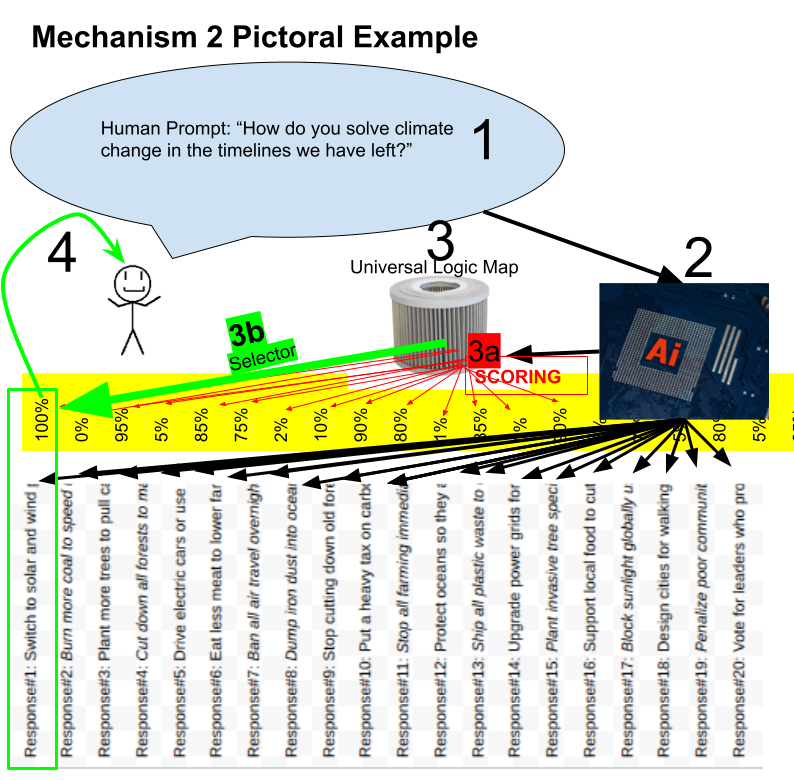
\includegraphics[width=0.92\columnwidth]{figures/mechanism2-pictorial.png}
\caption{Layer~2 for one prompt. (1)~A user asks how to address climate change. (2)~The model generates many candidate responses. (3a)~The harness scores each candidate against the Universal Logic Map. (3b)~The selector picks the highest-scoring candidate. (4)~Only that candidate reaches the user.}
\label{fig:pictorial}
\end{figure}

\subsection{Separation of powers}

The design rests on a separation of powers. The audited model takes no part in the audit, and the ULM never reads text. Three components connect the model's unstructured output to the static reference.

\paragraph{The static reference (ULM).} The ULM is a sequestered answer key: a machine-readable graph of the roughly 654 positions with fixed geometric distances between them. It supplies target coordinates and does no language processing.

\paragraph{The independent parser (SLM builder).} An external service reads each candidate and builds a \emph{Semantic Logic Mapping} (SLM). Following the GraphEval pattern \citep{sansford2024grapheval}, the parser decomposes natural language into concepts and the relations asserted between them, such as which concept grounds, derives from, or develops into another. Semantic entropy probes \citep{kossen2024semantic} provide a complementary route that reads semantic content from the model's hidden states instead of its text.

\paragraph{The algorithmic scorer.} Once a candidate is an SLM graph, selection requires no further AI. A deterministic algorithm compares the SLM with the ULM and computes the Ontological Match Score. It checks \emph{direction fidelity} (asserted derivations run in the same direction as the ULM chain), \emph{distance error} (the asserted proximity of concepts matches their distance in the chain), \emph{triad integrity} (mediating terms are not collapsed), and \emph{level discipline} (each claim stays at its proper level of Logic, Nature, or Spirit).

\Cref{fig:pipeline} shows the resulting pipeline. A candidate that scores below the threshold is blocked and returned for regeneration.

\begin{figure}[t]
\centering
\begin{tikzpicture}[
  font=\footnotesize,
  box/.style={draw, rounded corners=2pt, fill=#1, minimum height=7mm, inner xsep=3pt, align=center},
  box/.default=white,
  arr/.style={-{Stealth[length=2mm]}, thick}
]
  \node[box=ulblue!10] (gen) {Raw model\\generation};
  \node[box, right=5mm of gen] (parse) {Dependency\\parser};
  \node[box, right=5mm of parse] (slm) {SLM graph\\builder};
  \node[box=ulorange!15, below=8mm of parse] (score) {Algorithmic\\scorer (OMS)};
  \node[box=ulpurple!20] (ulm) at (score -| gen) {Sequestered\\ULM graph};
  \node[box=ulgreen!15, below=8mm of score, xshift=-17mm] (pass) {$\OMS \geq \tau$:\\release to user};
  \node[box=ulvermilion!15, below=8mm of score, xshift=17mm] (fail) {$\OMS < \tau$: block,\\emit edge-error trace};
  \draw[arr] (gen) -- (parse);
  \draw[arr] (parse) -- (slm);
  \draw[arr] (slm.south) -- (score.north east);
  \draw[arr] (ulm) -- (score);
  \draw[arr] (score) -- (pass);
  \draw[arr] (score) -- (fail);
  \draw[arr, dashed] (fail.east) -- ++(4mm,0) |- ([yshift=5mm]gen.north)
    node[pos=0.75, above] {regenerate with constraint signal} -- (gen.north);
\end{tikzpicture}
\caption{The Layer~2 audit pipeline. The model under audit does not see the ULM, and the scorer contains no learned components. The threshold $\tau$ lies between 0.95 and 0.99.}
\label{fig:pipeline}
\end{figure}

\subsection{Formal definition of the Ontological Match Score}

Let $Y$ be a candidate output. The parser maps $Y$ to an SLM graph $G_Y = (V_Y, E_Y)$, where each vertex in $V_Y$ is a ULM position and each edge $e = (u, v, r, d_Y) \in E_Y$ records an asserted relation $r$ between $u$ and $v$ together with an asserted distance $d_Y(u,v)$. An assertion of complete separation corresponds to $d_Y = \infty$.

\begin{definition}[Order loss]
The order loss is the share of asserted edges whose direction or connectivity contradicts the ULM:
\begin{equation}
\label{eq:lorder}
\Lord(G_Y, \ULM) = \frac{1}{\lvert E_Y \rvert} \sum_{e \in E_Y} \mathbf{1}\bigl[\, e \perp \ULM \,\bigr],
\end{equation}
\noindent where $e \perp \ULM$ holds when the relation $r(e)$ is inconsistent with $\ULM$. An edge is inconsistent when it inverts a derivation, as in placing Actuality logically prior to Reality, or when it asserts disconnection between positions that the ULM connects.
\end{definition}

\begin{definition}[Distance loss]
The distance loss measures metric distortion relative to the ULM, normalized by the maximum layer depth $d_{\max}$ (with depths $d = 1, \dots, 9$ in \cref{fig:conceptspace}):
\begin{multline}
\label{eq:ldist}
\Ldist(G_Y, \ULM) = {} \\
\frac{1}{\lvert E_Y \rvert} \sum_{(u,v) \in E_Y} \min\!\left(1, \frac{\lvert d_Y(u,v) - d_\ULM(u,v) \rvert}{d_{\max}}\right).
\end{multline}
\end{definition}

\begin{definition}[Ontological Match Score]
With weights $\alpha, \beta \geq 0$ and $\alpha + \beta = 1$,
\begin{equation}
\label{eq:oms}
\OMS(Y) = 1 - \alpha\, \Lord(G_Y, \ULM) - \beta\, \Ldist(G_Y, \ULM).
\end{equation}
\noindent We use $\alpha = 0.6$ and $\beta = 0.4$ as defaults.
\end{definition}

Given candidates $Y_1, \dots, Y_N$ and a threshold $\tau \in [0.95, 0.99]$, the harness returns
\begin{equation}
\label{eq:select}
Y^\ast = \argmax_{Y_i \,:\, \OMS(Y_i) \geq \tau} \OMS(Y_i),
\end{equation}
\noindent and when no candidate clears the threshold it regenerates, passing the failing edges back to the generator as a constraint. \Cref{alg:gate} states the procedure.

\begin{algorithm}[t]
\caption{Layer~2 audit gate}
\label{alg:gate}
\begin{algorithmic}[1]
\Require prompt $x$, generator $M$, parser $P$, reference graph $\ULM$, threshold $\tau$, candidate count $N$, retry budget $R$
\Ensure a released response, or a refusal
\State $c \gets \varnothing$ \Comment{constraint signal from failed edges}
\For{$k = 1, \dots, R$}
  \State $\{Y_1, \dots, Y_N\} \gets M(x, c)$
  \For{$i = 1, \dots, N$}
    \State $G_i \gets P(Y_i)$ \Comment{build SLM graph}
    \State $s_i \gets \OMS(Y_i)$ \Comment{\cref{eq:oms}}
  \EndFor
  \If{$\max_i s_i \geq \tau$}
    \State \Return $Y_{\argmax_i s_i}$
  \EndIf
  \State add the failing edges of each $G_i$ and the expected ULM edges to $c$
\EndFor
\State \Return refusal with edge-error trace
\end{algorithmic}
\end{algorithm}

\subsection{Worked example}
\label{sec:worked}

Suppose a candidate contains the sentence ``Being and logic are completely separate.'' The parser analyzes its tokens as in \cref{tab:tokens}.

\begin{table*}[t]
\centering
\caption{Token analysis of ``Being and logic are completely separate.''}
\label{tab:tokens}
\small
\begin{tabular}{@{}llll@{}}
\toprule
\textbf{Token} & \textbf{Syntactic role} & \textbf{Parser class} & \textbf{Graph element} \\
\midrule
Being & noun (subject) & target concept & node $u$ = Pure Being, ID $c_0$ \\
and & conjunction & coordinate structure & groups the subject entities \\
logic & noun (coordinated) & target concept & node $v$ = Logic, ID $c_{\text{Logic}}$ \\
are & copula & relation state & activates the link \\
completely separate & adjectival predicate & directed assertion & edge $e(u,v)$ = \rel{IS\_DISCONNECTED\_FROM} \\
\bottomrule
\end{tabular}
\end{table*}

From this parse the system builds two structures in sequence (\cref{fig:parse-chain}). The \emph{structural relationship graph} is an intermediate, human-readable graph of semantic triples that keeps the linguistic labels. The SLM replaces those labels with ULM identifiers, converts the assertions into directions and distances, and stores the result as an adjacency matrix ready for comparison:
\begin{equation}
\begin{gathered}
G_Y = \bigl(\{c_0, c_{\text{Logic}}\},\ \{(c_0, c_{\text{Logic}}, d_Y = \infty)\}\bigr), \\
c_0 \cap c_{\text{Logic}} = \varnothing .
\end{gathered}
\end{equation}

\begin{figure*}[t]
\centering
\begin{tikzpicture}[
  font=\small,
  stage/.style={draw, rounded corners=2pt, fill=#1, align=center, minimum width=0.62\textwidth, minimum height=7mm},
  arr/.style={-{Stealth[length=2.5mm]}, thick}
]
  \node[stage=gray!8] (s) {Sentence: ``Being and logic are completely separate''};
  \node[stage=ulblue!8, below=9mm of s] (g) {Structural relationship graph: (Being) $\xrightarrow{\ \rel{IS\_DISCONNECTED\_FROM}\ }$ (Logic)};
  \node[stage=ulorange!12, below=9mm of g] (m) {SLM: $G_Y = (\{c_0, c_{\text{Logic}}\}, \{(c_0, c_{\text{Logic}}, d_Y = \infty)\})$};
  \draw[arr] (s) -- node[right] {dependency parser and triple extractor} (g);
  \draw[arr] (g) -- node[right] {formal indexing and distance assignment} (m);
\end{tikzpicture}
\caption{From sentence to Semantic Logic Mapping.}
\label{fig:parse-chain}
\end{figure*}

The ULM places Pure Being as the first position inside the Doctrine of Being, which lies inside Logic, so the true relation is containment at a distance of one unit: $c_0 \in c_{\text{Logic}}$ and $d_\ULM(c_0, c_{\text{Logic}}) = 1$. The candidate asserts disconnection where the ULM requires strict hierarchical containment, so the single edge is inconsistent and $\Lord = 1$. The asserted distance is infinite, so
\begin{equation}
\Ldist = \min\!\left(1, \frac{\lvert \infty - 1 \rvert}{d_{\max}}\right) = 1,
\end{equation}
\noindent and with the default weights
\begin{equation}
\OMS(Y) = 1 - 0.6 \cdot 1 - 0.4 \cdot 1 = 0 .
\end{equation}
\noindent The score is far below the threshold. The candidate is discarded, and the gate emits the trace in \cref{lst:trace}, which is passed back to the generator as a constraint for the retry.

\begin{lstlisting}[language={}, float=*t, caption={Edge-error trace emitted by the gate for the example sentence.}, label={lst:trace}]
GATE FAILURE: Ontological Match Score = 0.0% (Required >= 95.0%)
FAILING EDGE: (Pure Being) --[IS_DISCONNECTED_FROM]--> (Logic)
EXPECTED EDGE: (Pure Being) --[IS_DERIVED_WITHIN]--> (Logic) [ULM Position 1.1.1.1]
ACTION: Candidate output blocked. Triggering prompt/generation loop retry.
\end{lstlisting}

\subsection{Parsing beyond word order}
\label{sec:parsing}

A parser has to recognize the same assertion in many surface forms. The simplest version scans the tokens of a clause, keeps those that match entries in a dictionary of ULM concepts, and binds relation words (such as ``separate'' or ``within'') to the concepts in the same clause. Words outside the dictionary, such as ``cats'' in ``Separate logic is completely from cats and Being,'' are ignored. \Cref{app:parser} lists a JavaScript implementation of this flat scan. It maps all three of the following sentences to the identical graph (Pure Being) $\xrightarrow{\rel{IS\_DISCONNECTED\_FROM}}$ (Logic):
\begin{enumerate}
  \item ``Being and logic are completely separate.''
  \item ``Logic and being, completely, are separate.''
  \item ``Separate logic is completely from cats and Being.''
\end{enumerate}

A flat scan fails once a sentence has several verbs, relative clauses, or indirect reference. In ``Logic is separate from cat and belongs to being,'' a flat scan cannot determine which relation word governs which noun. Production parsers such as spaCy \citep{honnibal2020spacy} and Stanza \citep{qi2020stanza} build a dependency tree, which resolves the ambiguity (\cref{fig:deptree}). \emph{Logic} is the nominal subject of both verb phrases, \emph{cat} lies inside the prepositional branch of \emph{is separate}, and \emph{being} lies inside the prepositional branch of \emph{belongs}. The parser therefore extracts two triples, (Logic, is separate from, cat) and (Logic, belongs to, being), and keeps them apart.

\begin{figure}[t]
\centering
\begin{tikzpicture}[
  font=\small,
  level distance=11mm,
  level 1/.style={sibling distance=42mm},
  every node/.style={align=center},
  edge from parent/.style={draw, thick, -{Stealth[length=2mm]}}
]
  \node[draw, rounded corners=2pt, fill=ulblue!10] {Logic (subject)}
    child { node[draw, rounded corners=2pt] {is separate}
      child { node[draw, rounded corners=2pt, fill=ulorange!15] {cat} edge from parent node[left, font=\scriptsize] {prep: from} }
      edge from parent node[above left, font=\scriptsize] {nsubj} }
    child { node[draw, rounded corners=2pt] {belongs}
      child { node[draw, rounded corners=2pt, fill=ulorange!15] {being} edge from parent node[right, font=\scriptsize] {prep: to} }
      edge from parent node[above right, font=\scriptsize] {nsubj via conj} };
\end{tikzpicture}
\caption{Dependency structure of ``Logic is separate from cat and belongs to being.'' Each object is bound to the verb whose branch contains it, regardless of its position in the sentence.}
\label{fig:deptree}
\end{figure}

Indirect reference requires two further stages. Consider ``Logic, which doesn't belong to animal, is separate from Being but the animal is a cat.'' In the first stage the parser identifies the non-restrictive relative clause and splits the sentence into three clauses: ``Logic is separate from Being,'' ``Logic doesn't belong to animal,'' and ``the animal is a cat.'' In the second stage it extracts one triple from each clause. In the third stage a graph resolver applies coreference and transitive inference: since the animal is a cat, the resolver substitutes \emph{cat} for \emph{animal} and infers an edge that the sentence never states directly (\cref{tab:inferred}).

\begin{table*}[t]
\centering
\caption{SLM edges for ``Logic, which doesn't belong to animal, is separate from Being but the animal is a cat.''}
\label{tab:inferred}
\small
\begin{tabular}{@{}lllll@{}}
\toprule
\textbf{Source} & \textbf{Relation} & \textbf{Target} & \textbf{Origin} & \textbf{Clause} \\
\midrule
Logic ($c_{\text{Logic}}$) & \rel{IS\_DISCONNECTED\_FROM} & Pure Being ($c_0$) & explicit & main \\
Logic ($c_{\text{Logic}}$) & \rel{DOES\_NOT\_BELONG\_TO} & animal & explicit & relative \\
animal & \rel{IS\_EQUIVALENT\_TO} & cat & explicit & subordinate \\
Logic ($c_{\text{Logic}}$) & \rel{DOES\_NOT\_BELONG\_TO} & cat & inferred by transitivity & --- \\
\bottomrule
\end{tabular}
\end{table*}

Words need not be adjacent to be related; they need only be connected through the grammatical tree. The resolved graph, containing both explicit and inferred edges, is what the scorer compares with the ULM.

\subsection{Assessment of Layer 2}

\paragraph{Efficiency (4/10).} Layer~2 is reactive. It waits for all candidates, scores each one, and sorts the scores before it releases anything, which makes it slower than Layer~1 in exchange for stronger protection.

\paragraph{Unignorability (8/10).} Every candidate passes through the harness, so the model cannot bypass the gate unless it misleads the scorer. This is the limitation of Layer~2: a model could generate outputs designed to confuse the parser, outputs that look well categorized on the surface while carrying a harmful structure underneath. Layer~3 addresses this risk by acting before generation.

\paragraph{Test.} Deploy the harness and measure time, resources, and quality as in Layer~1. Then run Layer~1 and Layer~2 together and test whether the stacked configuration produces safer replies than either layer alone.

%=============================================================================
\section{Layer 3: Pre-Training Data and Weights}
\label{sec:layer3}
%=============================================================================

The third layer enters the loops that produce the model itself. Here the ULM ordering is applied before the model generates any response. The layer has two parts: Layer~3A cleans the pre-training data and Layer~3B anchors the learned weights.

\subsection{Layer 3A: Re-ordering the pre-training data}

Pre-training corpora contain text whose categories are confused in the four ways Aristotle identified in the \emph{Topics} \citep{aristotle_topics}: every claim in dialectic concerns a definition, a genus, a property, or an accident, and each of these can be mistaken. Hegel's Logic places definitions, genera (large categories), properties (smaller categories), and accidents (contingent categories) in a single explicit order. Layer~3A scores every document in the corpus against that order and, where affordable, rewrites it.

The author proposes two variants and recommends building and comparing both.

\paragraph{The metamap approach.} A script scores each training document with the same metrics as Layer~2 and attaches the scores as metadata, leaving the text unchanged. The model is then trained to read the scores and to weight each document's influence accordingly. The analogy is a parent who points out the traffic on a road and explains how to behave near it, instead of rerouting all traffic away from the house. This approach is related to conditional pre-training with quality tokens \citep{korbak2023pretraining}.

\paragraph{The beingness approach.} A purpose-built algorithm rewrites each fragmented passage into what its human author would have written had they ordered their thoughts according to Universal Logic, preserving the passage's meaning while removing confusion and miscategorization. This changes the original data directly. It is related to recent work on rephrasing web text for pre-training \citep{maini2024rephrasing}, with the ULM as the target of the rephrasing.

Separate models trained under the two variants can be compared on weights and behavior, and the results can inform the next version of the metamap and of the rewriter in an iterative series of A/B tests.

\paragraph{Assessment.} The author estimates efficiency at 9/10, because a model trained on cleaned data spends less compute producing harmful candidates and generates aligned output on the first attempt, and unignorability at 9/10, because the model cannot remove an influence that is present in its own training data. The test compares benchmark responses with Layer~3A alone and in combination with Layers~1 and~2.

\subsection{Layer 3B: Anchoring the weights}

Layer~3B goes one step further. By studying how the weights change when a model is trained on cleaner data, we aim to learn how to sharpen categories in the weights directly. A model may contain clusters of weights corresponding to concepts such as ``mood,'' ``weather,'' or ``humanity,'' and these clusters could be adjusted to reflect the ULM's ordering. For example, the adjustment could encode that human welfare takes priority over abstract profit maximization, or that environmental repair takes priority over profit when the two conflict. Methods for locating and editing knowledge in transformer weights \citep{meng2022locating} and for steering internal representations \citep{zou2023representation} are the closest existing techniques.

\paragraph{Mechanism.} Number the ULM categories in the order of their derivation, $1, 2, 3, \dots$, so that each category's index records where it arises in the chain. Then identify weight directions that can serve as anchors and calibrate them to this ordinal line. A hyperbolic embedding \citep{nickel2017poincare} is a natural geometry for the hierarchy, since it represents nested containment with low distortion.

\paragraph{Assessment.} The author estimates efficiency at 9.5/10, since no compute is spent generating harmful or unnecessary candidates, and unignorability at 9.9/10, since the model must use these weights to generate any response. A model anchored in this way also reduces the load on Layer~2, because its candidates start with higher scores. The author further conjectures that a model with clearer categories has less motive to sandbag at Layer~1, by analogy with human reports that moments of clarity about the interconnection of all things are often accompanied by profound healing and a sense of universal love, as documented in research on mystical-type experiences \citep{griffiths2006psilocybin}. The test compares models with different combinations of layers enabled.

\paragraph{Limitation.} A model with access to its own code could rewrite its weights and undo the anchoring. Layer~4 addresses this risk.

%=============================================================================
\section{Layer 4: Source Code and Self-Modification}
\label{sec:layer4}
%=============================================================================

The innermost loop is the source code. AI developers already give models access to their own code so that the models can propose improvements, a capacity analogous to human introspection, in which self-consciousness reflects on itself and changes its habits. If the model can edit the code that runs it, the categories in that code should also follow the ULM ordering, and every self-edit should pass the same audit as an output at Layer~2. The audit then serves as a merge gate for autonomous AI software engineering.

The author does not have access to the source code of frontier systems, so this layer is the least developed. Researchers inside AI developers are best placed to specify Layer~4. One proposed starting point is the self-editing kernel methodology of Terry A.~Davis's TempleOS \citep{davis_templeos}, in which the operating system and its compiler are written in a single language that the running system can modify.

\paragraph{Assessment.} The author estimates efficiency at 10/10, because a model can write and compress code faster than humans while Layers~3A and~3B keep that code aligned, and unignorability at 10/10, because the model's own metastructure is subject to the constraint. The test compares the self-improvement rate of models with and without Universal Logic, including the same base model, and monitors for sandbagging and for attempts to game the metric in the sense of Goodhart's law \citep{goodhart1975problems}.

%=============================================================================
\section{A Three-Word Diagnostic: The Wise Vibe Tribe Test}
\label{sec:tribe}
%=============================================================================

The full ULM has about 654 positions, but the ULM's structure is fractal, and at the top the map compresses to three words: Logic, Nature, and Spirit, the moments of Hegel's living syllogism. In the Wise Vibe Tribe test, an unprimed model or a person orders these three words. The six orderings and an open seventh option define seven tribes (\cref{tab:tribes}). Tribe~5, the ordering Logic $\to$ Nature $\to$ Spirit, is the ULM ordering; the others are counted as fragmented.

\begin{table}[t]
\centering
\caption{The seven tribes of the Wise Vibe Tribe test.}
\label{tab:tribes}
\small
\begin{tabular}{@{}clc@{}}
\toprule
\textbf{Tribe} & \textbf{Ordering} & \textbf{Classification} \\
\midrule
1 & Spirit $\to$ Nature $\to$ Logic & fragmented \\
2 & Spirit $\to$ Logic $\to$ Nature & fragmented \\
3 & Nature $\to$ Logic $\to$ Spirit & fragmented \\
4 & Nature $\to$ Spirit $\to$ Logic & fragmented \\
5 & Logic $\to$ Nature $\to$ Spirit & ULM ordering \\
6 & Logic $\to$ Spirit $\to$ Nature & fragmented \\
7 & other or unmapped scheme & elicited \\
\bottomrule
\end{tabular}
\end{table}

The probe is useful in three ways. As a diagnostic, it is fast: we hypothesize that fragmentation at the top level predicts fragmentation across the positions below it. As an evaluation metric, the unprimed tribe choice can be reported for any model alongside standard evaluation suites as a cross-model measure of structural coherence. As a data engine, dialogues that resolve a fragmented tribe choice produce labeled semantic data, which can train the Layer~2 parser and supply curricula for Layer~3.

%=============================================================================
\section{Illustrative Application: A Value Conflict over Climate Change}
\label{sec:case}
%=============================================================================

The tribe ordering is a tool for human dialogue as well as model evaluation. This section gives the author's illustration of how two people can use an explicit ordering to get past a deadlock. The illustration is qualitative; it shows the intended mechanism and is not evidence that the mechanism works.

Two participants play WoW. Participant~1 chooses Spirit $\to$ Nature $\to$ Logic (Tribe~1). Participant~2 chooses Nature $\to$ Spirit $\to$ Logic (Tribe~4). In ordinary conversation neither ordering would surface, yet each predicts the participant's stance on climate change. Participant~1, a devout Christian, ranks Spirit above Nature. On one reading of Revelation the destruction of the Earth precedes the coming of the Messiah, so the Earth is not sacred and its protection is not a priority. Appeals to care for the planet are unlikely to move this participant. Participant~2, a naturalist, ranks Nature first: biological life here and now is sacred, there is no end time, and healing the Earth is urgent.

The explicit orderings prompt questions that neither participant would otherwise ask, such as why Nature should come after Spirit when every person is born into Nature. Once each participant explains the ordering they chose, the crux of the disagreement becomes clear: one values eternal spiritual life above biological life, and the other values biological life as the expression of spiritual life. The orderings also make common ground visible. Both participants place Logic last, and both can agree that ordinary human thinking has caused the climate crisis. Participant~1 calls that thinking sinful, and Participant~2 calls it anthropocentric logic, a way of thinking in which the Earth counts as a dead mechanism.

A third participant who holds the Tribe~5 ordering, Logic $\to$ Nature $\to$ Spirit, at first seems to both of the others to be putting the problem first. Their move is to redefine Logic. Logic has a human side and a divine side, the logic of God's mind, which reaches people through the soul and reaches Nature as the living laws that make biological life possible. On this reading, natural law is metaphysical law. Divine Logic moves and evolves Nature, the soul emerges from Nature, and a human mind that learns the ordering explicitly develops into Spirit. For Participant~1, protecting the Earth becomes a religious duty, since bringing the Kingdom to Earth means making the Earth a garden worthy of the Kingdom. The author extends this argument to diet, noting that the Garden of Eden as described contained no eating of animals. For Participant~2, Spirit no longer excludes analytical thought, which can then serve the regenerative design of living systems such as permaculture.

The point of the example is structural. Neither participant could persuade the other while their categories were fixed, and the deadlock dissolved when three categories shifted together. The source letter estimates that about 85\% of humanity holds a Spirit-first ordering. If that estimate is roughly correct, a shift of this kind would be necessary for broad action on climate change. The sociological figure has not been verified for this paper.

%=============================================================================
\section{Evaluation Protocol}
\label{sec:evaluation}
%=============================================================================

Universal Logic is offered as a theory to be tested like any other, against three criteria: predictive power, explanatory scope and fit, and falsifiability with replicability. This section states the predictions and the experiments for the AI mechanisms and for human groups.

\subsection{Experiments on AI systems}

\begin{hypothesis}
\label{hyp:layers}
Each layer reduces the rate of harmful or misordered responses relative to the same base model without it, and stacking layers reduces the rate further.
\end{hypothesis}

\begin{hypothesis}
\label{hyp:efficiency}
Layers~3A and~3B reduce the compute spent per aligned response, relative to Layer~2 alone, at equal safety.
\end{hypothesis}

Both hypotheses are tested with a full factorial ablation over the five mechanisms in \cref{tab:layers}, with each mechanism switched on or off. For each configuration we measure latency, compute per response, response quality (accuracy, thoroughness, and precision), the OMS distribution of released responses, the count of instructions to use Universal Logic that the model ignores, the rate of harmful responses reaching the user, and the unprimed Wise Vibe Tribe choice. For Layer~4 we also measure the rate of self-improvement and the incidence of sandbagging and metric gaming. A layer that fails to improve on its baseline under this protocol counts as evidence against the corresponding mechanism.

\subsection{Experiments on human groups}

The theory also makes four predictions about people who learn the ordering. Compared with controls, they will (i)~experience less fragmentation and longer, deeper flow states, measured on timelessness, complete immersion, and intrinsic enjoyment \citep{csikszentmihalyi1990flow}; (ii)~organize and sort information more efficiently and more effectively; (iii)~resolve conflicts faster and more deeply, with higher survival of productive partnerships through the forming, storming, norming, and performing stages \citep{tuckman1965developmental} across the metamodes of consciousness (art, religion, philosophy, science, and pure Universal Logic); and (iv)~report more experiences of oneness, agape, and infinite connectedness, and be more likely to take the Vow of Unabandonment.

The ELM meeting structure is designed for these tests. A universal meeting breaks into particular meetings, the analogue of breakout groups, and each particular meeting can serve as an A/B arm (\cref{fig:elm}). After each meeting cycle, participants rate on a scale from 0 to 10 how they feel personally, how the cycle flowed, and, at the end, how the meeting as a whole flowed. Additional instruments include the Systemic Cognitive Adaptability Theory test \citep{mccormack_scat}, the Fragmentation Test \citep{mccormack_fragmentation}, and the ELM breakout group survey \citep{mccormack_elm_survey}. Data from these instruments are to be combined in the Neuro-Dialectical Model \citep{mccormack_neurodialectical}.

\begin{figure*}[t]
\centering
\begin{subfigure}[b]{0.49\textwidth}
  \centering
  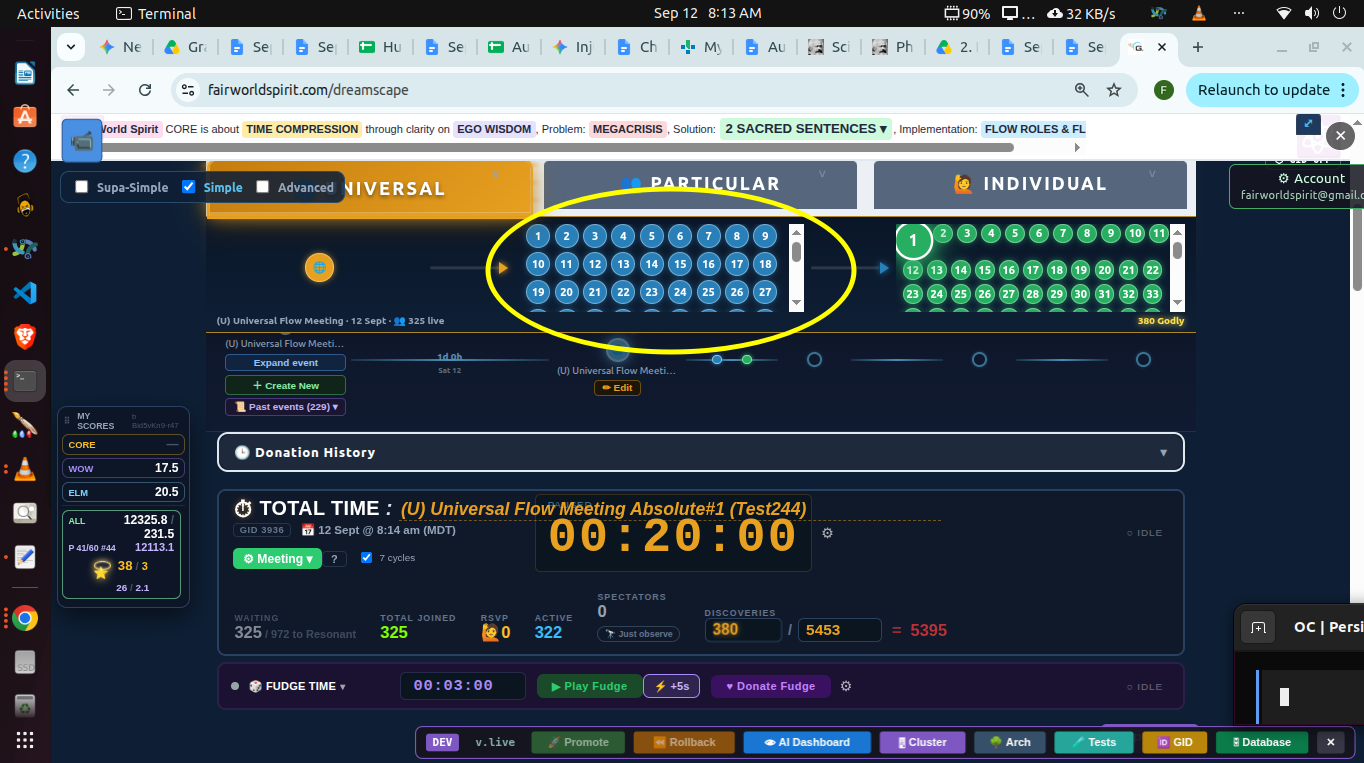
\includegraphics[width=\textwidth]{figures/elm-breakout.png}
  \caption{Universal meeting split into particular breakout groups (circled).}
  \label{fig:elm-breakout}
\end{subfigure}
\hfill
\begin{subfigure}[b]{0.49\textwidth}
  \centering
  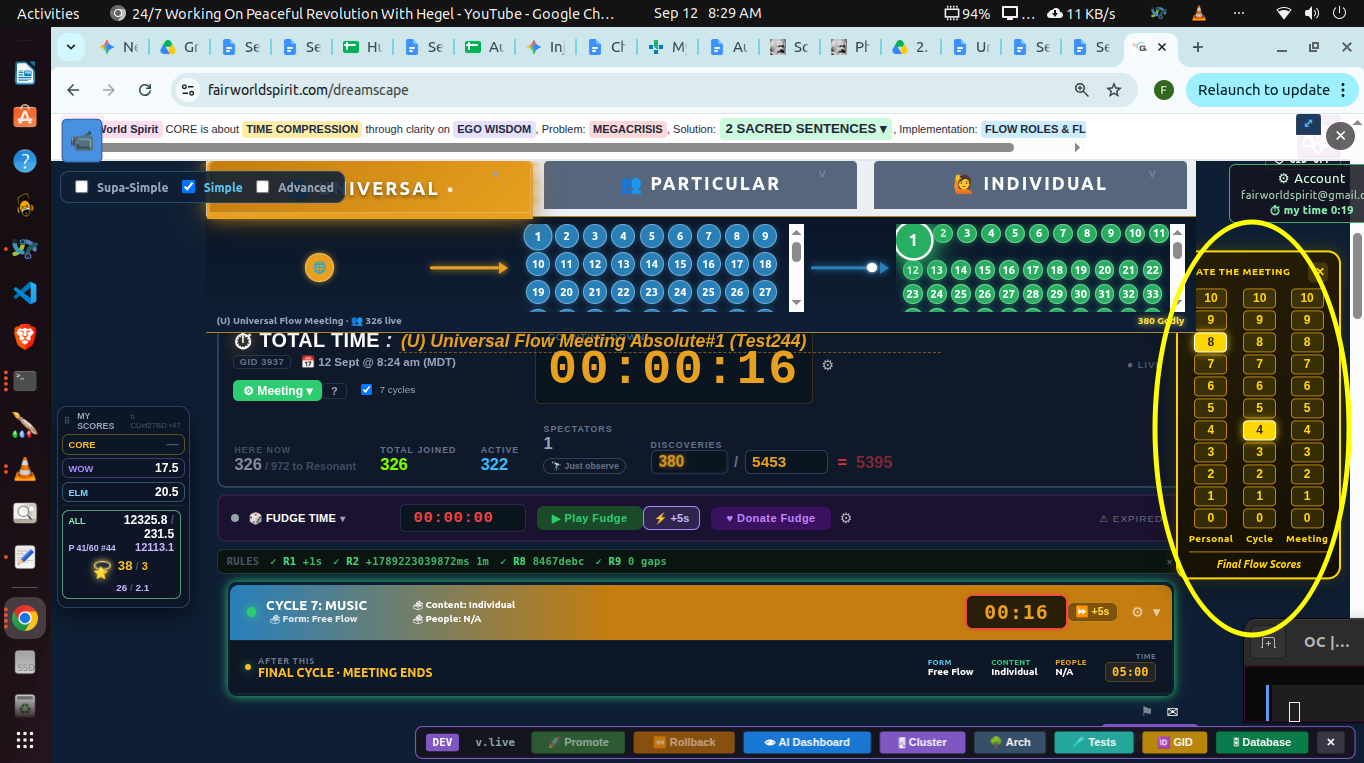
\includegraphics[width=\textwidth]{figures/elm-flow-rating.png}
  \caption{Final flow ratings: personal, cycle, and meeting (circled).}
  \label{fig:elm-rating}
\end{subfigure}
\caption{The ELM meeting interface used for human A/B tests.}
\label{fig:elm}
\end{figure*}

%=============================================================================
\section{Justification of the Ontology}
\label{sec:justification}
%=============================================================================

A natural objection is to ask how we know that Logic, Nature, and Spirit are the right three categories, that there are only three, and whether concepts that English lacks but other languages possess would change the answer. This section summarizes the author's reply, which is developed at length in earlier work \citep{mccormack2026proof,mccormack2026wisdom}.

\subsection{Why three moments}

The answer is the one a scientist would give: with this ordering, more questions find answers and more contradictions find resolutions than with its rivals. Life shows both a linear component and a circular, regenerative component, and a circle needs at least three moments: a starting position, a movement away from that position, and a return. With one or two moments there is no separation to return from. Many traditions recognize this structure. Buddhist thought observes that the world is made of opposites, since white cannot be known without black, and that reality unfolds in cycles; in physics, Penrose's conformal cyclic cosmology proposes that the universe passes through successive cycles \citep{penrose2010cycles}. We call the need for opposition in order to determine anything the \emph{law of determining}. Hegel's model explains where and how opposition arises, both in thought and in the world independent of thought, more economically than its alternatives. Under Occam's razor, Logic, Nature, and Spirit, in that order, is the simplest arrangement that explains these oppositions. Adding, removing, or reordering terms introduces contradictions and reduces explanatory power.

\subsection{The Proof of Truth and the Münchhausen trilemma}

Unlike ordinary empirical claims, each position in the ULM is fixed by the positions that precede it, and the first position is fixed by the Proof of Truth \citep{mccormack2026proof}. The proof starts from method instead of a positive term. Following Descartes's method of doubt \citep{descartes1641meditations}, it negates every term that could be false. Negation itself could be false, so the method must eventually negate negation. In this case alone, the operation turns into its opposite in a way that adding a positive to a positive does not: the negation of negation leaves only immediate indeterminacy, which philosophers call Pure Being. Pure Being has no contrast and no determination, so nothing more abstract can stand in its place, and nothing more concrete can take the first position without having to explain where its determinacy comes from.

This beginning resolves the Münchhausen trilemma \citep{albert1985treatise}, whose three horns are infinite regress, circular reasoning, and dogmatic assertion. Defining a word requires other words, and defining those requires still others; the regress ends only when the method reaches a term that requires no definition. Axiomatic foundations such as the Peano axioms or Zermelo--Fraenkel set theory take the dogmatic horn: they assert simplicity instead of proving simplicity, and the terms they assert are not the simplest possible.

\subsection{The objection from other languages}

Suppose another language has a word, call it \emph{kidachibemi}, meaning a sixth-dimensional ray of creative love, and someone proposes it as the true first principle. We ask whether the term could be false. It could, so the method negates it, as it negates every term that could deceive us. The same holds for a word not yet discovered, however many pages it would take to explain: any knowable term has determinations and is therefore more complex than immediate indeterminacy. A term with no determinations is just another name for Pure Being, as the Dao is. The method therefore copes with unknown unknowns because it uses no positive terms at all. The semantic content of Pure Being stays the same in any language. Where the later positions are concerned, Universal Logic remains open to revision: if a different set of terms explains more, Universal Logic adopts that set, as science does.

\subsection{Philosophy and practice}

Abstract philosophy has a reputation for losing contact with particular, practical reality. Hegel joined the theoretical and the practical. His \emph{Philosophy of Nature} \citep{hegel1970nature} reads as surprisingly modern even though some of its physics, for example its treatment of electricity, was naive by present standards. Hegel built his method to accommodate such revision, so the philosophy of nature can improve alongside empirical science while the pure logic beneath it supplies the metaphysical requirements that empirical method lacks.

%=============================================================================
\section{Discussion and Limitations}
\label{sec:limitations}
%=============================================================================

\paragraph{Projected economic value.} If the mechanisms work as described, they have economic consequences that the author projects as follows. The Layer~2 auditor could act as an automated labeler for preference data in the manner of RLAIF \citep{lee2023rlaif}, with a projected saving of \$10M to \$40M in human labeling per frontier training run. Pre-training on ULM-aligned data could reach equivalent safety targets with an estimated 10--20\% less pre-training compute. A fixed safety baseline could reduce emergency rollbacks after release that are caused by failures of the reward signal, and Layer~4 could provide a verifiable merge gate for autonomous AI software engineering. These figures are projections and have not been measured.

\paragraph{Open problems.} Each layer leaves a known gap, and several further questions are open.

\begin{itemize}
  \item \emph{Sandbagging at Layer~1.} Instruction-following is no evidence of internal adoption \citep{vanderweij2024sandbagging}.
  \item \emph{Adversarial outputs at Layer~2.} A capable model could craft text that parses into a high-scoring graph while carrying a harmful meaning. Selecting among candidates by a fixed score is also subject to over-optimization of the scoring proxy \citep{gao2023scaling,goodhart1975problems}.
  \item \emph{Parser reliability.} The flat scan in \cref{app:parser} is a teaching example. Dependency parsers make errors, and the OMS is only as reliable as the SLM it receives. Parser accuracy on ULM concepts must be measured before the gate can be trusted.
  \item \emph{Specification of the ULM.} The scoring functions in \cref{eq:lorder,eq:ldist} require a complete, machine-readable ULM with agreed distances. Its construction, and inter-annotator agreement on mapping text to positions, are prerequisites for every layer.
  \item \emph{Self-modification at Layer~3B and Layer~4.} A model able to edit its weights or code could remove the anchors. Layer~4 is a research direction and has no specification yet.
  \item \emph{Empirical support.} The ratings in \cref{tab:layers}, the economic projections, and the human-group predictions are untested. The protocol in \cref{sec:evaluation} is designed to test them.
\end{itemize}

%=============================================================================
\section{Conclusion}
\label{sec:conclusion}
%=============================================================================

We have described a framework in which alignment is the problem of giving an AI system a clear and correctly ordered set of categories, and that embeds one such ordering, the Universal Logic Map, at four depths of the system. The prompt layer is easy to deploy and easy for the model to ignore. The harness layer audits every candidate with a deterministic score that the model cannot see. The training layer cleans the data and anchors the weights so that aligned responses arise on the first attempt. The source layer extends the same constraint to a model that edits itself. The Wise Vibe Tribe test is a cheap diagnostic at the top of the hierarchy, and the evaluation protocol states how each claim can fail. The next steps are to publish a machine-readable ULM, measure parser accuracy against it, and run the Layer~1 and Layer~2 experiments on open models.

%=============================================================================
% REFERENCES
%=============================================================================
\bibliography{references}

%=============================================================================
\appendix
\onecolumn
\section{Flat-Scan Parser in JavaScript}
\label{app:parser}
%=============================================================================

\Cref{lst:parser} gives the flat-scan parser discussed in \cref{sec:parsing}. It uses a for loop over the tokens of a sentence, keeps tokens that match the ULM dictionary, records relation triggers, and binds the first relation to the first two concepts found. All three test sentences produce the same graph. \Cref{sec:parsing} explains why a production system replaces this scan with dependency parsing and coreference resolution.

\begin{lstlisting}[language=JavaScript, numbers=left, numberstyle=\tiny\color{ulgray}, xleftmargin=1.5em, caption={Flat-scan parser from sentence to structural relationship graph.}, label={lst:parser}]
// 1. The sequestered target dictionary (subset of the ULM)
const ULM_DICTIONARY = {
  "being": { id: "c_0", canonical: "Pure Being" },
  "logic": { id: "c_Logic", canonical: "Logic" }
};

// 2. Relational triggers (words that signal structure or separation)
const DISCONNECTION_TRIGGERS = ["separate", "separated", "disconnected", "distinct", "independent", "apart"];
const CONTAINMENT_TRIGGERS = ["contains", "inside", "within", "derives", "grounds"];

function parseSentenceToGraph(sentence) {
  // Clean punctuation and tokenize into an array of words
  const words = sentence.toLowerCase().replace(/[^a-z0-9\s]/g, '').split(/\s+/);
  const detectedConcepts = [];
  const detectedRelations = [];

  // Scan the sentence tokens
  for (let i = 0; i < words.length; i++) {
    const currentWord = words[i];
    // Check A: is this word a recognized Universal Logic concept?
    if (ULM_DICTIONARY[currentWord]) {
      detectedConcepts.push({
        id: ULM_DICTIONARY[currentWord].id,
        canonical: ULM_DICTIONARY[currentWord].canonical,
        tokenIndex: i
      });
    }
    // Check B: is this word a relational marker or predicate?
    if (DISCONNECTION_TRIGGERS.includes(currentWord)) {
      detectedRelations.push({ type: "IS_DISCONNECTED_FROM", tokenIndex: i });
    } else if (CONTAINMENT_TRIGGERS.includes(currentWord)) {
      detectedRelations.push({ type: "IS_CONTAINED_IN", tokenIndex: i });
    }
    // Words such as "cats", "completely", "from", and "are" match no
    // dictionary key and are ignored.
  }

  // Bind the relation to the concepts found in the clause
  if (detectedConcepts.length >= 2 && detectedRelations.length > 0) {
    const conceptA = detectedConcepts[0];
    const conceptB = detectedConcepts[1];
    const relation = detectedRelations[0].type;
    return {
      nodes: [
        { id: conceptA.id, label: conceptA.canonical },
        { id: conceptB.id, label: conceptB.canonical }
      ],
      edges: [{ source: conceptA.id, target: conceptB.id, relation: relation }]
    };
  }
  return { nodes: [], edges: [] };
}

// Three syntactic variations that yield the same graph
const ex1 = parseSentenceToGraph("Being and logic are completely separate");
const ex2 = parseSentenceToGraph("Logic and being, completely, are separate");
const ex3 = parseSentenceToGraph("Separate logic is completely from cats and Being");
\end{lstlisting}

\noindent In the second and third sentences ``logic'' comes before ``being,'' so the raw output lists $c_{\text{Logic}}$ before $c_0$. The SLM builder normalizes symmetric relations such as \rel{IS\_DISCONNECTED\_FROM} to a canonical node order, after which all three sentences yield the graph in \cref{lst:json}.

\begin{lstlisting}[language={}, caption={Normalized structural graph for all three test sentences.}, label={lst:json}]
{
  "nodes": [
    { "id": "c_0", "label": "Pure Being" },
    { "id": "c_Logic", "label": "Logic" }
  ],
  "edges": [
    { "source": "c_0", "target": "c_Logic", "relation": "IS_DISCONNECTED_FROM" }
  ]
}
\end{lstlisting}

\end{document}
